% This document holds the main content of the talk. It is included in
% the two global documumetns `Presentation.tex` and `Handout.tex` that
% are used to create the actual presentation as well as a two on one
% collated handout of the slides.
%
% All real content has to go to _this_ file!
%
% Last change: <Wed, 2022/02/09 16:12:37 arwagner l00lnxwagner.desy.de>
%
\mode<handout>{%
    \usepackage{pgf}
    \usepackage{pgfpages}
    \pgfpagesuselayout{2 on 1}[a4paper,border shrink=5mm]
}
\mode<presentation>{%
    \usetheme{DESY}
}
% Setup for Beamer
\usepackage{hyperxmp}
% \usepackage[pdfa]{hyperref}
\usepackage{luatextra}
\usepackage{wasysym}
\usepackage{eurosym}
\usepackage{bookmark}
\usepackage{graphicx}
\usepackage{fontspec}

% Force beamer to use Arial. Without this it will fall back to
% Libertine in all ``normal'' text areas. It seems they are not easily
% accessible from the templates.
\usefonttheme{professionalfonts} % using non standard fonts for beamer
\setmainfont[Mapping=tex-text]{Arial}
\setsansfont[Mapping=tex-text]{Arial}

%% Force Arial for math as well like strict CD.
%% However, usually TeX defaults just look way better
% \usepackage{unicode-math}
% \setmathfont{Arial} % for math symbols, can be any other OpenType math font
% \setmathfont[range=\mathup]  {Arial}
% \setmathfont[range=\mathbfup]{Arial Bold}
% \setmathfont[range=\mathbfit]{Arial Bold Italic}
% \setmathfont[range=\mathit]  {Arial Italic}

\usepackage[ngerman,english]{babel}
\usepackage{xspace}
\usepackage{tikz}
\usepackage{fancyvrb}
\tikzset{%
  every overlay node/.style={%
    %draw=black,fill=white,rounded corners,anchor=north west,
    draw=fzjlightblue,fill=fzjgray30,rounded corners,anchor=north west,
  },
}
% Usage:
% \tikzoverlay at (-1cm,-5cm) {content};
% or
% \tikzoverlay[text width=5cm] at (-1cm,-5cm) {content};
\def\tikzoverlay{%
   \tikz[baseline,overlay]\node[every overlay node]
}%

% General new commands an macros
\renewcommand{\emph}[1]{\structure{#1}}

\newcommand{\link}[2]{\href{#1}{~#2}}

\newcommand{\jointwo}{\href{http://join2.de}{\textbf{JOIN$^2$}\xspace}}

\newcommand{\BibTeX}{Bib\TeX}

\newcommand{\Inspec}{{\texttt{Inspec}}\xspace}
\newcommand{\WoS}{{\texttt{Web of Science}}\xspace}
\newcommand{\Scopus}{\texttt{Scopus}\xspace}
\newcommand{\arxiv}{{\texttt{arXiv.org}}\xspace}
\newcommand{\pubmed}{{\texttt{pubmed}}\xspace}

\newcommand{\JabRef}{\link{http://jabref.sf.net}{JabRef}\xspace}
\newcommand{\Companion}[1]{\textit{\link{http://julib.fz-juelich.de/uhtbin/field-search-sort/001/PBYR/213964}{\LaTeX{} Companion}, #1}\xspace}
\newcommand{\pkg}[1]{\emph{\texttt{#1}}\xspace}

\newcommand{\neutralino}{\ensuremath{\tilde{\chi}^0}\xspace}

% general colour definitions
\newcommand{\smallgray}[1]{{\tiny\emph{#1}}}

\newcommand{\idR}{i.~d.~R.\xspace}
\newcommand{\va}{v.~a.\xspace}
\newcommand{\sa}{s.~a.\xspace}
\newcommand{\zB}{z.~B.\xspace}
\newcommand{\zT}{z.~T.\xspace}
\newcommand{\eg}{e.~g.\xspace}

\newcommand{\bs}[1]{\texttt{$\backslash$#1}}
\newcommand{\command}[2]{\texttt{\bs{#1}\{#2\}}}

\newcommand{\invenio}{\href{http://invenio-software.org}{\raisebox{-0.5em}{\includegraphics[height=1.5em]{pictures/Logo_invenio}}}}
\newcommand{\github}{\href{http://github.com}{%
	\raisebox{-1em}{\includegraphics[height=2.0em]{pictures/Octocat}}%
	\raisebox{-0.5em}{\includegraphics[height=1.5em]{pictures/GitHub_Logo}}}}

\newcommand{\newitem}{\raisebox{-0.7ex}{\includegraphics[height=3ex]{img/new_icon}}}
\newcommand{\newicon}{\raisebox{-1.1ex}{\includegraphics[height=4ex]{img/new_icon}}}
\newcommand{\verytiny}[1]{{\fontsize{3}{4}\selectfont{#1}}}

\newcommand{\DESYWord}{%
\raisebox{0.0px}{%
	\usebeamercolor[fg]{title}{\textbf{DESY}}%
	\usebeamercolor[fg]{subtitle}{\textbf{.}}
}\hspace*{0.2em}
}

\newcommand{\MailTo}[1]{\href{mailto:#1}{#1}}
\newcommand{\DOIlink}[1]{\href{https://doi.org/#1}{\emph{#1}}}
\newcommand{\ORCiD}[1]{
\includegraphics[height=1.5ex]{img/orcid}\,\href{https://www.orcid.org/#1}{#1}}

%%--%% % http://tex.stackexchange.com/questions/16447/beamer-top-aligning-columns-within-a-top-aligned-fram
\makeatletter
\newenvironment{topitemize}{%
   \setlength{\topsep}{0pt}
   \setlength{\partopsep}{0pt}
   \renewcommand*{\@listi}{\leftmargin\leftmargini \parsep\z@ \topsep\z@ \itemsep\z@}
   \let\@listI\@listi
   \itemize
}{\enditemize}
\makeatother

%------------------- Begin of edit -----------------------------------
%
% Adopt the follwing values according to your needs.
%
% Note: improving metadata also improves visibility. Time spent here
% might pay of later. Search engines love keywords, abstracts and
% sensible titles.
%
%     Make sure to submit your talk to the publications database
%         to get a DOI, to make it citable and OpenAccess!
%
\newcommand{\TITLE}{Machine Learning in Quantum Mechanics}     % Title of talk       
\newcommand{\SUBTITLE}{Normalizing Flows for Computing Molecular Vibrational Wave Functions}                 % Subtitle
\newcommand{\AUTHOR}{Nicolas Mendoza}        % your name
\newcommand{\EMAIL}{snmendozav@gmail.com} % your email
\newcommand{\ORCID}{0000--0001--5561--1392}   % your ORCiD
\newcommand{\PHONE}{+49--152--2768--2024}      % your phone number
\newcommand{\GROUP}{CMI}          % your group
\newcommand{\URL}{http://library.desy.de}     % your groups page
\newcommand{\DOI}{10.3204/PUBDB-20YY-nnnn}    % submit and release in pubdb to get a DOI
\newcommand{\INSTITUTE}{DESY} % not used in CD 2018
\newcommand{\CITY}{Hamburg}                      % City of talk
\newcommand{\DATE}{07.09.2022}                % Date of Talk

% To improve visibility - add metadata to the PDF
% - Add sensible keywords describing the topic
% - Add the abstract (one line, no breaks it is just for indexing)
% - Adopt the licence of your work

\hypersetup{%
	pdfkeywords        = {keyword} {keyword} {keyword},
	pdfsubject         = {Abstract},
	pdfcopyright       = {CC-BY},
	pdflicenseurl      = {http://creativecommons.org/licenses/by/4.0/},
	%% pdfcopyright       = {CC-BY-NC-SA},
	%% pdflicenseurl      = {http://creativecommons.org/licenses/by-nc-sa/4.0/},
	pdftitle           = {\TITLE}
	pdfcreator         = {\AUTHOR},
	pdfcaptionwriter   = {\AUTHOR},
	pdfcontactaddress  = {Notkestraße 85},
	pdfcontactcity     = {Hamburg},
	pdfcontactpostcode = {22607},
	pdfcontactcountry  = {Germany},
	pdfcontactemail    = {\EMAIL},
	pdfcontacturl      = {\URL},
	pdflang            = {en},
	bookmarksopen      = true,
	bookmarksopenlevel = 3,
	hypertexnames      = false,
	linktocpage        = true,
	plainpages         = false,
	breaklinks
}

%------------------- End of edit -------------------------------------

% Derive internal values from above data

\author{\AUTHOR}
\title{\TITLE}
\subtitle{\SUBTITLE}
\institute{}  % not used by DESY CD 2018
\date{\CITY, \DATE}



%---------------------------------------------------------------------

\begin{document}

\maketitle

% Add a licencse statement to all pages. Adopt this if any other
% licences is used!

%-% CC-BY-NC-SA 4
%-% \setbeamertemplate{slide counter}[showall][]
%-% \setbeamertemplate{footer element1}{%
%-%     \href{http://creativecommons.org/licenses/by-nc-sa/4.0/}{
\includegraphics[height=3ex]{img/CCBYNCSA}}
%-% }

% CC-BY 4, current suggetion for scientific content
\setbeamertemplate{slide counter}[showall][]
\setbeamertemplate{footer element1}{%
    \href{http://creativecommons.org/licenses/by/4.0/}{
\includegraphics[height=3ex]{img/CCBY}}
}

%----------------------------------------------------------------------
% Add manual table of contents
% Two column example
% -% \begin{frame}
% -% \frametitle{Overview}
% -%   \begin{columns}
% -%       \begin{column}{0.4\textwidth}
% -%           \hspace*{-0.97cm}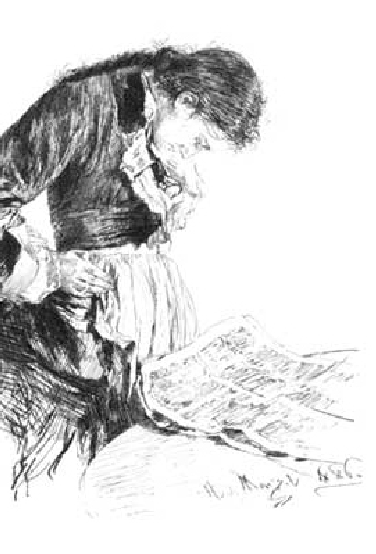
\includegraphics[height=\textheight]{img/menzel}
% -%       \end{column}
% -%       \begin{column}{0.5\textwidth}
% -%           \begin{itemize}[<+->]
% -%               \item {Section}
% -%               \item {Section}
% -%           \end{itemize}
% -%       \end{column}
% -%   \end{columns}
% -% \end{frame}

\begin{frame}
\frametitle{Overview}
  \begin{itemize}[<+->]
      \item {Introduction}
      \item {Physics}
      \item {Machine Learning}
      \item {Mathematics}
  \end{itemize}
\end{frame}

\begin{frame}
    \frametitle{Overview}
    \begin{itemize}[<+>]
        \item {Introduction}
        \item {Physics}
        \item {Machine Learning}
        \item {Mathematics}
    \end{itemize}
\end{frame}
%----------------------------------------------------------------------
% Missuse parts as chapters according to DESY PR
\part[Part slide]{Introduction}
\makepart%

%----------------------------------------------------------------------
\section{\ldots}

% Add a sample slide with some math, some columns etc.
\begin{frame}[t,label=intro]
\frametitle{The Challenge}

\begin{itemize}[<+->]
    \setlength\itemsep{.8em}
    \item Solving Schrödinger's Equation is \textbf{hard}
    \item Usually turn to numerical approximations
    \item \ldots but numerics have limitations
    \item Amountof data needed depends exponentially on $d$
\end{itemize}

\begin{columns}
    \begin{column}[t]{0.48\textwidth}
        \begin{itemize}[<+->]
            \setlength\itemsep{.8em}
            \item \textit{The Curse of Dimensionality}
            \item How do we improve dependency?
            \item More flexibility to our basis elements 
            \item Machine Learning comes into play
        \end{itemize}
    \end{column}
    \begin{column}[t]{0.48\textwidth}
        \begin{figure}
            \includegraphics[width=\textwidth]{example-image-a}
        \end{figure}
        % Hello there
    \end{column}
\end{columns}

% left aligned columns. Note that columns with smaller width are
% centred automatically

\end{frame}


%----------------------------------------------------------------------
% Thank you page is assembled from metadata.tex
\begin{frame}
\frametitle{Thank you!}
\vfill{}
\vspace*{3.5cm}

% check %-% comments for inclusion of a QR code. This is not official
% DESY CD.

\fontsize{8}{9}\selectfont
\begin{columns}
	\hspace*{-0.8em}
	\hspace*{-1em}  % comment if QR code is inserted
	%-% \begin{column}{0.75\textwidth}
	\begin{column}{\textwidth}
		\begin{tabular}{lll}
		\textbf{Contact}&\hspace*{0.5cm} & \\
						&\hspace*{0.5cm} & \\
		\hspace*{-0.4mm}Deutsches Elektronen-&\hspace*{0.5cm} & \AUTHOR\\
		\hspace*{-0.4mm}Synchrotron DESY&\hspace*{0.5cm} & \ORCiD{\ORCID}\\
							&\hspace*{0.5cm} & \GROUP\\
							&\hspace*{0.5cm} & \MailTo{\EMAIL}\\
		\hspace*{-0.4mm}www.desy.de			&\hspace*{0.5cm} & \PHONE\\
							&\hspace*{0.5cm} & \DOIlink{\DOI}\\
		\end{tabular}
	\end{column}
	%-% \begin{column}{0.24\textwidth}
	%-% 
\includegraphics[width=0.8\textwidth]{img/aw-vcf-QRCode}\\
	%-% 	{\tiny\textit{Typeset by lua\LaTeX}}
	%-% \end{column}
\end{columns}


\end{frame}

\end{document}
% Enable spell checker for vim
% setlocal spell spelllang=de
